%%%%%%%%%%%%%%%%%%%%%%%%%%%%%%%%%%%%%%%%%
% Beamer Presentation
% LaTeX Template
% Version 2.0 (10/06/16)
%
% Attention:
% 0. The self-defined font is used, because 'Calibri' is 
% not supported in the latex font packages. 'LuaLatex'
% should be used.
% 1. This template has been generated according to 
% the Power Point template of LUMC in 2016. 
% 2. This is generated purely with images as the 
% background.
% 3. The bullet point color was used purely for personal 
% preference. 
% 4. Any more adding to the template are welcome. 
% 5.In order to use the navigation bar, the title 
% for each section should not be to long. 
% 6.Adding animation is possible. I prefer to add another
% pdf file with:
% \animategraphics[parameters]{1}{fname}{startnum}{endnum}
% 7. This is my first template, the files might be not  
% well organized, sorry for that. 
% 
% Author:
% Shengnan Liu
% sliu729@gmail.com
% Division Medical imaging processing, 
% Leiden University Medical Center
% 
%%%%%%%%%%%%%%%%%%%%%%%%%%%%%%%%%%%%%%%%%
% Modification Log:
% Generated by Shengnan Liu on 21-01-2016
% Cleaned up for further usage on 10-06-2016
%%%%%%%%%%%%%%%%%%%%%%%%%%%%%%%%%%%%%%%%%
\documentclass{beamer}
\title{Here you can put a very very very very very very long title}
\date[today]{\today}
\author[Name]{You name}
\institute[Department]{Leiden University Medical Center}
\usetheme{lumc}% theme
\usepackage{multicol} % 
%\usepackage{animate}  % animation
\usepackage{amsmath,amsfonts,amssymb} % This makes the equations appears better 
\begin{document}
%The title
\begin{frame}
\titlepage
\end{frame}


% Adding note that cannot be seen
\note[itemize]{
\item Good morning everyone. Today I would like to present the work that were submitted to SPIE proceeding photonics west. 
\item point 2
}

% The outline
\begin{frame}{Outline}
\tableofcontents
\end{frame}

\section{Introduction}% for adding section
\subsection{subtitle1}
\begin{frame}{title}
\begin{center}
\includegraphics<1>[height=10cm]{im/chd1}%<*> is used to control the playing order  
\includegraphics<2>[height=10cm]{im/chd1}%
\par
Illustration from Libby P: Inflammation in Atherosclerosis. Nature 202;420:868%it is always nice to add the source of the images 
\end{center}
\end{frame}

\begin{frame}{~}
\begin{block}{another template}
~~~~~~~~~~~~\\
~~\\
\begin{itemize}
\item<1->Point 1
\item<2->Point 2
\end{itemize}
\end{block}
\end{frame}

\begin{frame}{Title}
\begin{columns}[onlytextwidth]
\column{0.02\textwidth}
\column{.45\textwidth}
\includegraphics<1->[height = 10cm]{im/ivoct}\par
(http://www.bioopticsworld.com/topics/cardiology.htm)% Reference 
\column{.45\textwidth}
\begin{itemize}
\item<1-> Point 1
\item<2-| alert@2> Point 2% you may want to highlight it
\end{itemize}
\end{columns}
\end{frame}

\subsection{subtitle2}

\subsection{subtitle3}
\begin{frame}
\begin{block}{challenges}
~~~~~~~~~~~~\\
~~\\
~~
YOU MAY WANT TO INVOLVE SOME ATTENTION?
\end{block}
\end{frame}

\subsection{subtitle 4}
% \begin{frame}{The aim of the study}
% \studygoal% This is a flow chart defined in beamerthemelumc.sty. You can try to play with it if you are familiar with 'tikz' package.
% \end{frame}

\section{Method}
\begin{frame}{Method with equation and image}
\begin{block}{with a block name}
\centering
$\log a \cong  \beta_2\text{\bf ln~}
b + \beta_1 x_t + \beta_0$\par
~~\\
~~\\
~~\\
~~\\
\centering
\includegraphics<2>[width = 10cm]{im/chd1}
~~\\
~~\\
~~\\
~~\\
\end{block}
\end{frame}


\begin{frame}{Data and results}
\subsection{Data Description}
\begin{block}{Data Description}
~~\\
~~\\
Description of your data ???
~~\\
~~\\
\end{block}
\subsection{Results}% you can start a subsection in a slice
\begin{block}{Results}
\centering
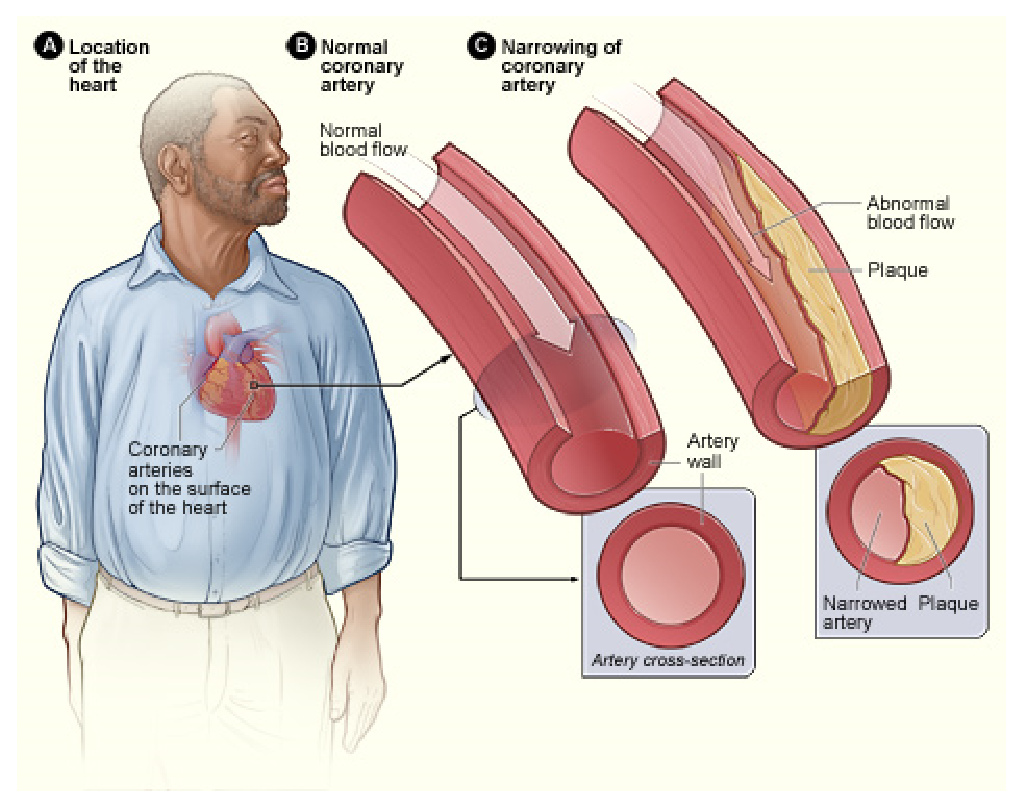
\includegraphics[height = 10cm]{im/chd1}
\end{block}
\end{frame}


\begin{frame}{statistical results with table}
\begin{block}{Results}
~~\\
\begin{center}
\resizebox{\textwidth}{!}{\normalsize\bf
\begin{tabular}{lp{1.8cm}lp{1.6cm}lp{1.6cm}lp{1.4cm}lp{1.2cm}lp{1.4cm}lp{2cm}lp{2cm}}
{\centering Estimates of ...$^*$}\\
\hline 
Parameter~ & Estimate & ~~Std.Error~ & $df$ & ~$t$~ & $Sig.$ &
\multicolumn{2}{l}{$95\%$ Confidence Interval} \\
~ & ~ & ~ & ~ & ~ & ~ & Lower & Upper\\
~ & ~ & ~ & ~ & ~ & ~ & Bound & Bound\\
\cline{7-8} $\beta _0$ & 0.123 & ~~~0.123 & 0.123 & 0.123 & 0.123 &
0.123 & 0.123\\
$\beta _1$ & ${\bf -0.002}$ & ~~~0.123 & 0.123 & ${\bf -0.123}$ & 0.123 & ${\bf -0.123}$ & ${\bf -0.123}$\\
$\beta _2$ & 0.123 & ~~~0.123 & 0.123 & 0.123 & 0.123 & 0.123 & 0.123\\%{\bf} operator for negative numbers 
\hline\multicolumn{8}{l}{*. some comments.}\\
\hline
\end{tabular}
}
~~\\
~~\\
\resizebox{\textwidth}{!}{\normalsize\bf
\begin{tabular}{lp{1.8cm}lp{1.6cm}lp{1.6cm}lp{1.4cm}lp{1.2cm}lp{1.4cm}lp{2cm}lp{2cm}}
{\centering Estimates of ...$^{**}$}\\
\hline Parameter & ~ & ~~Estimate & $Std.$ & Wald Z & $Sig.$ &
\multicolumn{2}{l}{$95\%$ Confidence Interval} \\
~ & ~ & ~ & ~ & ~ & ~ & Lower & Upper\\
~ & ~ & ~ & ~ & ~ & ~ & Bound & Bound\\
\cline{7-8} Residual & ~ & ~~~0.123 & 0.123 & 0.123 & 0.123 & 0.123 & 0.123\\
Intercept[variable1] & Variance & ~~~0.123 & 0.123 & 0.123 & 0.123 & 0.123 & 0.123\\
Intercept[variable2] & Variance & ~~~0.123 & 0.123 & 0.123 & 0.123 & 0.123 & 0.123\\
\hline\multicolumn{8}{l}{**. some comments.}\\
\hline
\end{tabular}
}
\end{center}
~~\\
~~\\
\end{block}
\end{frame}

\section{Other}
\subsection{Other method}
\begin{frame}{Other method}
\begin{block}{~}
\centering
$a =
\frac{b\cdot e^c}{d}$
\end{block}
\end{frame}

\subsection{Other Result}
\begin{frame}{Other Result}
\centering
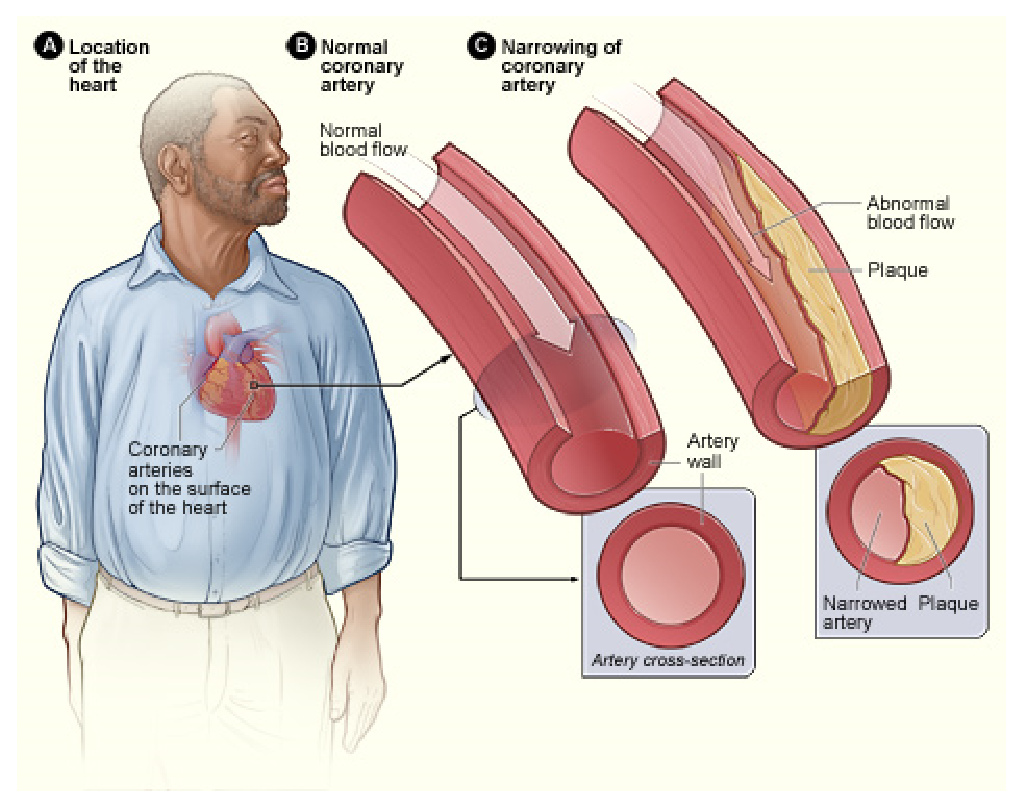
\includegraphics[width = 13cm]{im/chd1}
\end{frame}

\section{Discussion}
\begin{frame}{~}
\begin{columns}[onlytextwidth]
\column{0.02\textwidth}
\column{.9\textwidth}
\begin{block}{Discussion}
~~\\
~~\\
\begin{itemize}
\item point 1
\vskip0.5cm
\item point 2
\vskip0.5cm
\item point 3 
\vskip0.5cm
\item point 4
\vskip0.5cm
\item point 5
\vskip0.5cm
\item point ...
\vskip0.5cm
~
\end{itemize} 
\end{block}
\column{0.02\textwidth}
\end{columns}
\end{frame}
%\section{Update of the work}
\section{Acknowledgment}
\begin{frame}{Acknowledgement}
\begin{columns}[onlytextwidth]
\column{0.02\textwidth}
\column{.45\textwidth}
\begin{block}{Group name}
\begin{itemize}
\vskip0.5cm
\item name 
\vskip0.5cm
\item name 
\end{itemize}
\vskip1.7cm
~
\end{block}
\vskip1cm 
\begin{block}{group name}
\vskip0.5cm 
\begin{itemize}
\item name
\vskip0.5cm
\item name 
\end{itemize}
\vskip1.7cm
~
\end{block}

\column{.45\textwidth}
\begin{block}{Organizations}
\vskip0.5cm 
\begin{itemize}
\item name 
\vskip0.5cm
\item name 
\vskip0.5cm
\end{itemize}
\end{block}
\vskip1cm
\begin{block}{Poortgebouw Group}
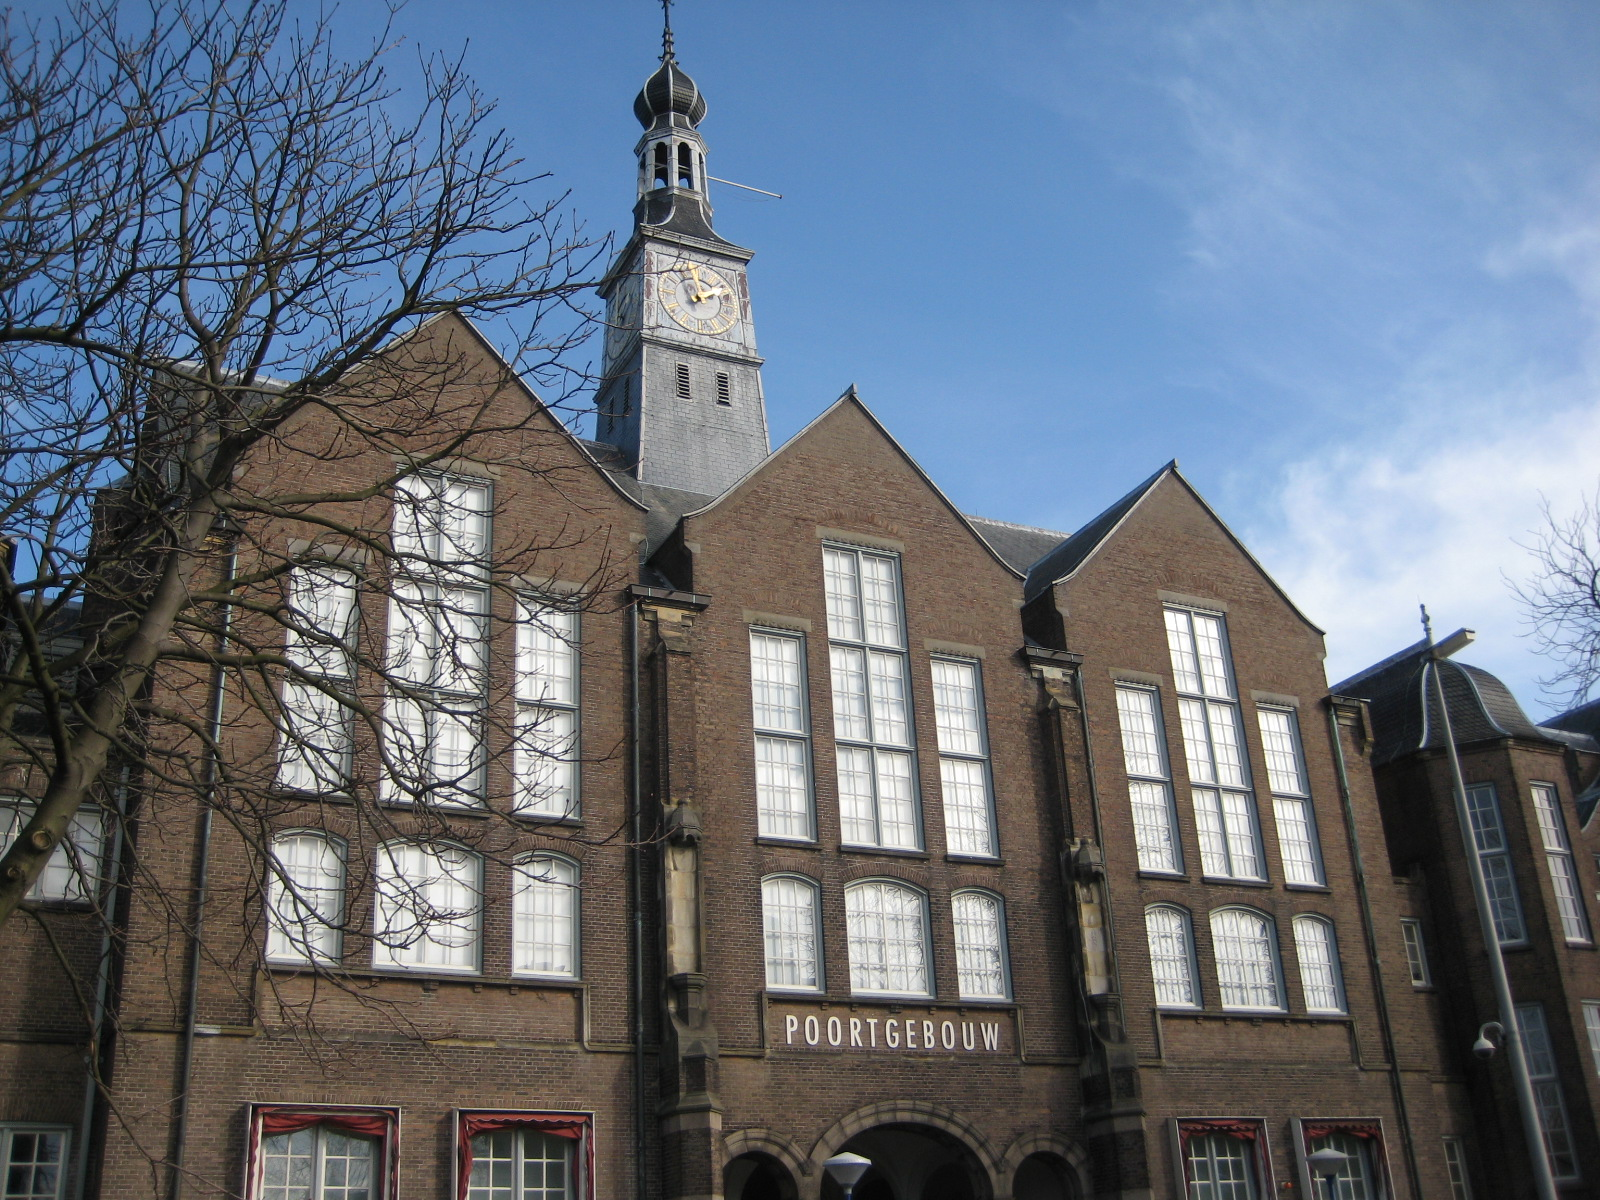
\includegraphics[height=0.4\textheight]{poort.jpg}%
\end{block}
\column{0.02\textwidth}
\end{columns}


\end{frame}
\begin{frame}[label={lastframe}]
\end{frame}
\end{document}
